%%%%%%%%%%%%%%%%%%%%%%%%%%%%%%%%%%%%%%%%%%%%%%%%%%%%%%%%%%%%%%%%%%%%%%%%%%%%%%%%
%2345678901234567890123456789012345678901234567890123456789012345678901234567890
%        1         2         3         4         5         6         7         8

%\documentclass[letterpaper, 10 pt, conference]{ieeeconf}  % Comment this line out
                                                          % if you need a4paper
\documentclass[letterpaper, 10pt, conference]{ieeeconf}      % Use this line for a4
                                                          % paper

\IEEEoverridecommandlockouts                              % This command is only
                                                          % needed if you want to
                                                          % use the \thanks command
\overrideIEEEmargins
% See the \addtolength command later in the file to balance the column lengths
% on the last page of the document

%\setlength{\topmargin}{0.46in}


% The following packages can be found on http:\\www.ctan.org
\usepackage{graphics} % for pdf, bitmapped graphics files
\usepackage[dvips]{graphicx} % for eps
\usepackage{epsfig} % for postscript graphics files
%\usepackage{mathptmx} % assumes new font selection scheme installed
\usepackage{times} % assumes new font selection scheme installed
\usepackage{amsmath} % assumes amsmath package installed
%\usepackage{amssymb}  % assumes amsmath package installed
\usepackage{wasysym}
\usepackage{color}
\usepackage{algorithmic}
\usepackage{tensor}
\usepackage{leftidx}

%\usepackage[dvips, bookmarks=false, colorlinks=true, pdftitle={Hak-Humanoids2010}]{hyperref}
\newcommand{\mbf}[1]{{\mathbf{#1}}}
\newcommand{\dpartial}[2]{\frac{\partial{#1}}{\partial{#2}}}
\DeclareMathOperator*{\argmin}{arg\,min\,} 


\title{\LARGE \bf
Reverse engineering task recognition and disambiguation on humanoid robot
}

\author{Sovannara Hak, Nicolas Mansard, Jean-Paul Laumond% <-this % stops a space
  \thanks{7 av col Roche, F-31077 Toulouse, France, Universit\'e de Toulouse; UPS, INSA, INP,
    ISAE: {\tt\small sovannara.hak@laas.fr, nicolas.mansard@laas.fr, jpl@laas.fr}.}
  \thanks{This work was supported by a grant from the R-Blink Project, Contract
    ANR-08JCJC-0075-01.}  }


\begin{document}

\maketitle
\thispagestyle{empty}
\pagestyle{empty}


%%%%%%%%%%%%%%%%%%%%%%%%%%%%%%%%%%%%%%%%%%%%%%%%%%%%%%%%%%%%%%%%%%%%%%%%%%%%%%%%
\begin{abstract}
Reverse engineering the motion.
\end{abstract}

\section{Experimentation on the robot}

\subsection{Experimental setup}
Robot HRP2
Motion capture system: markers, skeleton, joint angle trajectory

A motion capture system is used in order to have an external observation of the robot.
The motion capture system used is composed of 10 digital cameras. A set of 50 markers
are placed on the robot to record a motion (see figure~\ref{fig:hrp2Markers}). The data collected from those markers
are used to build a virtual skeleton that match the kinematic structure of the robot.
\begin{figure}[t]
\centering
\begin{tabular}{cc}
\parbox[c]{3.6cm}{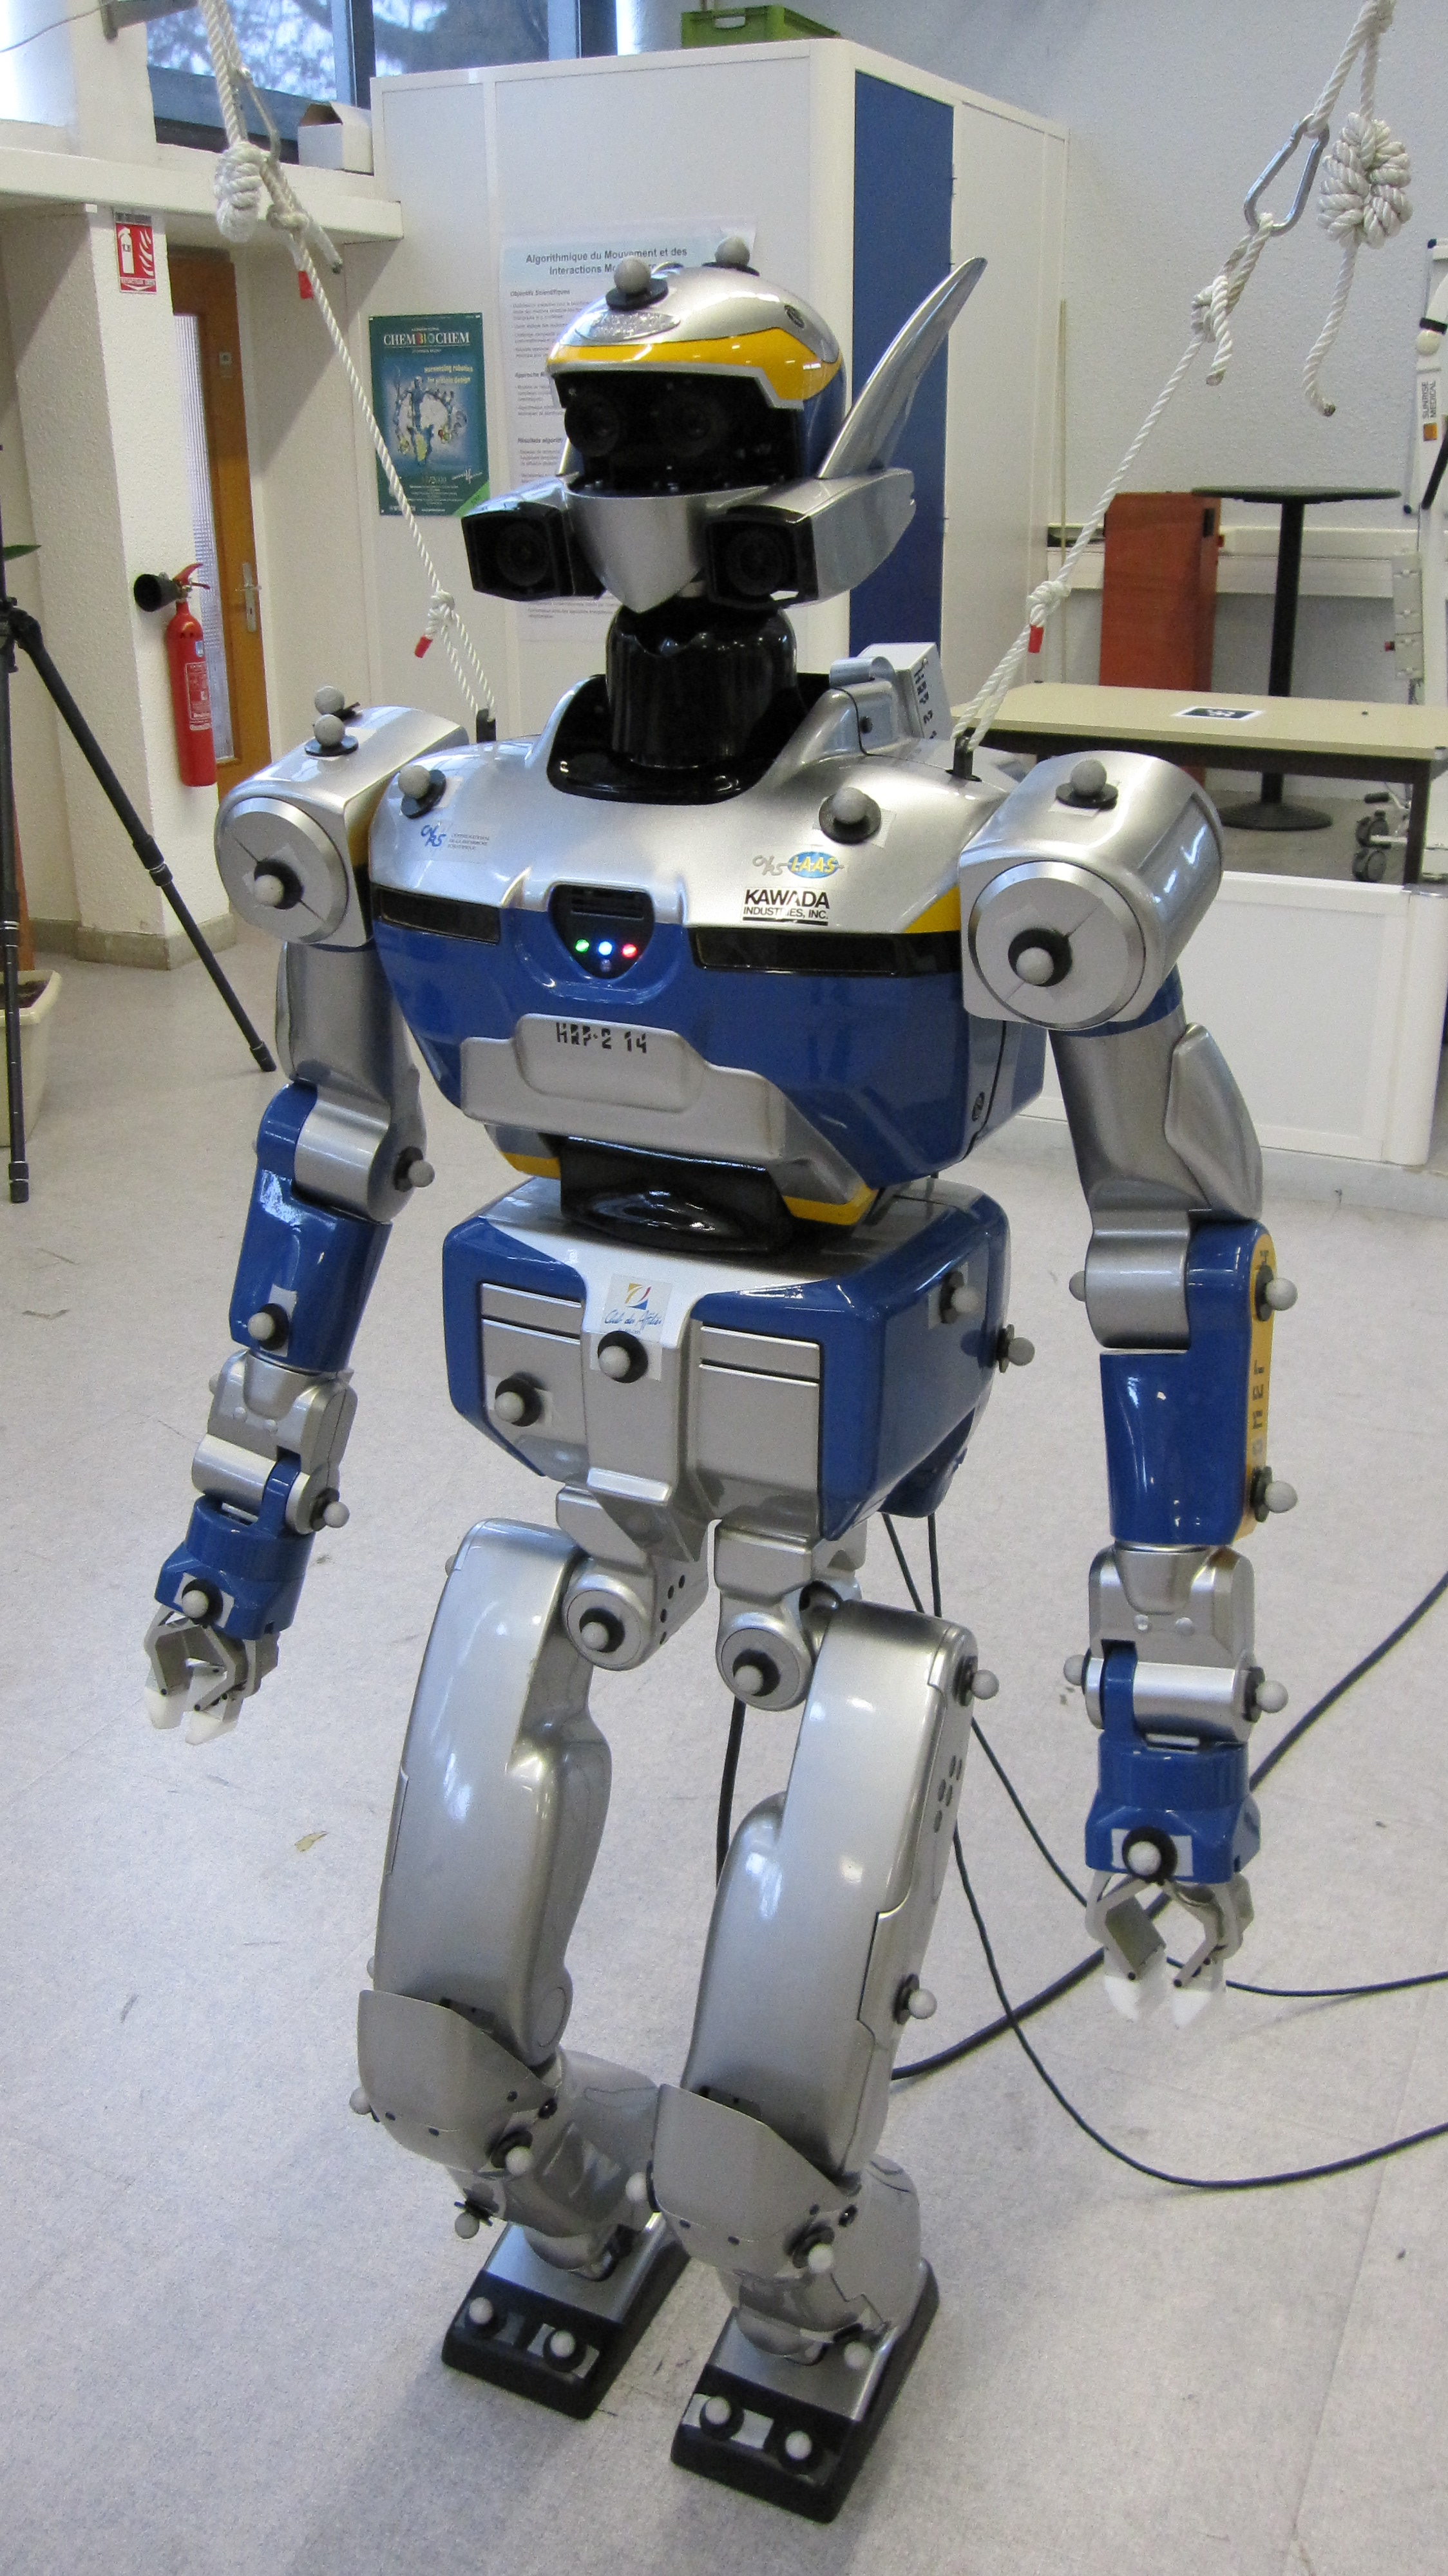
\includegraphics[width=\linewidth]{img/hrp2Markers.ps}} &
\parbox[c]{3.45cm}{\includegraphics[width=\linewidth]{img/skel.ps}} \\
\end{tabular}
\caption{Markers set and virtual skeleton of HRP2.}
\label{fig:hrp2Markers}
\end{figure}

The computation of the trajectory of the motion in the joint angle space
of the robot is done by optimization.
\begin{equation}
\mbf{q}^*_i = \underset{\mbf{q}_i}\argmin \Vert K_W\tensor[^{0M}]{R}{_{iM}}K_i \ominus \tensor[^W]{R}{_{iQ}}(\mbf{q}_i) \Vert ^2\\
\label{mocapOpti}
\end{equation}

Joint angle trajectory are needed by the algorithm.

In this experimentation, the robot has to move both of his
hands toward desired positions.


\begin{itemize}
\item Both hands versus one hand
\item Grab blind, Grab and look
\item Grab, screw
\end{itemize}

\subsection{Right hand VS Both hands motion}
\begin{figure*}[t]
\begin{tabular*}{0.9\textwidth}{@{\extracolsep{\fill}}cc}
  \resizebox{.4\textwidth}{!} {
	% GNUPLOT: LaTeX picture with Postscript
\begingroup
  \makeatletter
  \providecommand\color[2][]{%
    \GenericError{(gnuplot) \space\space\space\@spaces}{%
      Package color not loaded in conjunction with
      terminal option `colourtext'%
    }{See the gnuplot documentation for explanation.%
    }{Either use 'blacktext' in gnuplot or load the package
      color.sty in LaTeX.}%
    \renewcommand\color[2][]{}%
  }%
  \providecommand\includegraphics[2][]{%
    \GenericError{(gnuplot) \space\space\space\@spaces}{%
      Package graphicx or graphics not loaded%
    }{See the gnuplot documentation for explanation.%
    }{The gnuplot epslatex terminal needs graphicx.sty or graphics.sty.}%
    \renewcommand\includegraphics[2][]{}%
  }%
  \providecommand\rotatebox[2]{#2}%
  \@ifundefined{ifGPcolor}{%
    \newif\ifGPcolor
    \GPcolortrue
  }{}%
  \@ifundefined{ifGPblacktext}{%
    \newif\ifGPblacktext
    \GPblacktexttrue
  }{}%
  % define a \g@addto@macro without @ in the name:
  \let\gplgaddtomacro\g@addto@macro
  % define empty templates for all commands taking text:
  \gdef\gplbacktext{}%
  \gdef\gplfronttext{}%
  \makeatother
  \ifGPblacktext
    % no textcolor at all
    \def\colorrgb#1{}%
    \def\colorgray#1{}%
  \else
    % gray or color?
    \ifGPcolor
      \def\colorrgb#1{\color[rgb]{#1}}%
      \def\colorgray#1{\color[gray]{#1}}%
      \expandafter\def\csname LTw\endcsname{\color{white}}%
      \expandafter\def\csname LTb\endcsname{\color{black}}%
      \expandafter\def\csname LTa\endcsname{\color{black}}%
      \expandafter\def\csname LT0\endcsname{\color[rgb]{1,0,0}}%
      \expandafter\def\csname LT1\endcsname{\color[rgb]{0,1,0}}%
      \expandafter\def\csname LT2\endcsname{\color[rgb]{0,0,1}}%
      \expandafter\def\csname LT3\endcsname{\color[rgb]{1,0,1}}%
      \expandafter\def\csname LT4\endcsname{\color[rgb]{0,1,1}}%
      \expandafter\def\csname LT5\endcsname{\color[rgb]{1,1,0}}%
      \expandafter\def\csname LT6\endcsname{\color[rgb]{0,0,0}}%
      \expandafter\def\csname LT7\endcsname{\color[rgb]{1,0.3,0}}%
      \expandafter\def\csname LT8\endcsname{\color[rgb]{0.5,0.5,0.5}}%
    \else
      % gray
      \def\colorrgb#1{\color{black}}%
      \def\colorgray#1{\color[gray]{#1}}%
      \expandafter\def\csname LTw\endcsname{\color{white}}%
      \expandafter\def\csname LTb\endcsname{\color{black}}%
      \expandafter\def\csname LTa\endcsname{\color{black}}%
      \expandafter\def\csname LT0\endcsname{\color{black}}%
      \expandafter\def\csname LT1\endcsname{\color{black}}%
      \expandafter\def\csname LT2\endcsname{\color{black}}%
      \expandafter\def\csname LT3\endcsname{\color{black}}%
      \expandafter\def\csname LT4\endcsname{\color{black}}%
      \expandafter\def\csname LT5\endcsname{\color{black}}%
      \expandafter\def\csname LT6\endcsname{\color{black}}%
      \expandafter\def\csname LT7\endcsname{\color{black}}%
      \expandafter\def\csname LT8\endcsname{\color{black}}%
    \fi
  \fi
  \setlength{\unitlength}{0.0500bp}%
  \begin{picture}(7200.00,5040.00)%
    \gplgaddtomacro\gplbacktext{%
      \csname LTb\endcsname%
      \put(1342,704){\makebox(0,0)[r]{\strut{} 0}}%
      \put(1342,1194){\makebox(0,0)[r]{\strut{} 0.01}}%
      \put(1342,1684){\makebox(0,0)[r]{\strut{} 0.02}}%
      \put(1342,2174){\makebox(0,0)[r]{\strut{} 0.03}}%
      \put(1342,2665){\makebox(0,0)[r]{\strut{} 0.04}}%
      \put(1342,3155){\makebox(0,0)[r]{\strut{} 0.05}}%
      \put(1342,3645){\makebox(0,0)[r]{\strut{} 0.06}}%
      \put(1342,4135){\makebox(0,0)[r]{\strut{} 0.07}}%
      \put(1474,484){\makebox(0,0){\strut{} 0}}%
      \put(2245,484){\makebox(0,0){\strut{} 2}}%
      \put(3016,484){\makebox(0,0){\strut{} 4}}%
      \put(3787,484){\makebox(0,0){\strut{} 6}}%
      \put(4557,484){\makebox(0,0){\strut{} 8}}%
      \put(5328,484){\makebox(0,0){\strut{} 10}}%
      \put(6099,484){\makebox(0,0){\strut{} 12}}%
      \put(6870,484){\makebox(0,0){\strut{} 14}}%
      \put(440,2542){\rotatebox{90}{\makebox(0,0){\strut{}$\Vert \dot{q}\Vert$ (rad/s)}}}%
      \put(4172,154){\makebox(0,0){\strut{}$t$ (s)}}%
      \put(4172,4710){\makebox(0,0){\strut{}Right hand motion - Com task}}%
    }%
    \gplgaddtomacro\gplfronttext{%
      \csname LTb\endcsname%
      \put(5883,4207){\makebox(0,0)[r]{\strut{}$J^+ \dot{e}_{com}$}}%
      \csname LTb\endcsname%
      \put(5883,3987){\makebox(0,0)[r]{\strut{}Model}}%
    }%
    \gplbacktext
    \put(0,0){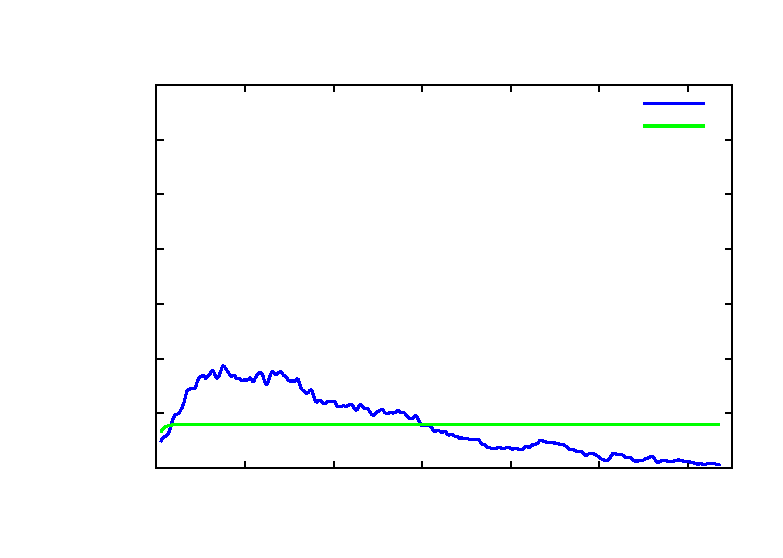
\includegraphics{img/exp1/R/invJerror_taskCom_0}}%
    \gplfronttext
  \end{picture}%
\endgroup

    }                           &
  \resizebox{.4\textwidth}{!} {
	% GNUPLOT: LaTeX picture with Postscript
\begingroup
  \makeatletter
  \providecommand\color[2][]{%
    \GenericError{(gnuplot) \space\space\space\@spaces}{%
      Package color not loaded in conjunction with
      terminal option `colourtext'%
    }{See the gnuplot documentation for explanation.%
    }{Either use 'blacktext' in gnuplot or load the package
      color.sty in LaTeX.}%
    \renewcommand\color[2][]{}%
  }%
  \providecommand\includegraphics[2][]{%
    \GenericError{(gnuplot) \space\space\space\@spaces}{%
      Package graphicx or graphics not loaded%
    }{See the gnuplot documentation for explanation.%
    }{The gnuplot epslatex terminal needs graphicx.sty or graphics.sty.}%
    \renewcommand\includegraphics[2][]{}%
  }%
  \providecommand\rotatebox[2]{#2}%
  \@ifundefined{ifGPcolor}{%
    \newif\ifGPcolor
    \GPcolortrue
  }{}%
  \@ifundefined{ifGPblacktext}{%
    \newif\ifGPblacktext
    \GPblacktexttrue
  }{}%
  % define a \g@addto@macro without @ in the name:
  \let\gplgaddtomacro\g@addto@macro
  % define empty templates for all commands taking text:
  \gdef\gplbacktext{}%
  \gdef\gplfronttext{}%
  \makeatother
  \ifGPblacktext
    % no textcolor at all
    \def\colorrgb#1{}%
    \def\colorgray#1{}%
  \else
    % gray or color?
    \ifGPcolor
      \def\colorrgb#1{\color[rgb]{#1}}%
      \def\colorgray#1{\color[gray]{#1}}%
      \expandafter\def\csname LTw\endcsname{\color{white}}%
      \expandafter\def\csname LTb\endcsname{\color{black}}%
      \expandafter\def\csname LTa\endcsname{\color{black}}%
      \expandafter\def\csname LT0\endcsname{\color[rgb]{1,0,0}}%
      \expandafter\def\csname LT1\endcsname{\color[rgb]{0,1,0}}%
      \expandafter\def\csname LT2\endcsname{\color[rgb]{0,0,1}}%
      \expandafter\def\csname LT3\endcsname{\color[rgb]{1,0,1}}%
      \expandafter\def\csname LT4\endcsname{\color[rgb]{0,1,1}}%
      \expandafter\def\csname LT5\endcsname{\color[rgb]{1,1,0}}%
      \expandafter\def\csname LT6\endcsname{\color[rgb]{0,0,0}}%
      \expandafter\def\csname LT7\endcsname{\color[rgb]{1,0.3,0}}%
      \expandafter\def\csname LT8\endcsname{\color[rgb]{0.5,0.5,0.5}}%
    \else
      % gray
      \def\colorrgb#1{\color{black}}%
      \def\colorgray#1{\color[gray]{#1}}%
      \expandafter\def\csname LTw\endcsname{\color{white}}%
      \expandafter\def\csname LTb\endcsname{\color{black}}%
      \expandafter\def\csname LTa\endcsname{\color{black}}%
      \expandafter\def\csname LT0\endcsname{\color{black}}%
      \expandafter\def\csname LT1\endcsname{\color{black}}%
      \expandafter\def\csname LT2\endcsname{\color{black}}%
      \expandafter\def\csname LT3\endcsname{\color{black}}%
      \expandafter\def\csname LT4\endcsname{\color{black}}%
      \expandafter\def\csname LT5\endcsname{\color{black}}%
      \expandafter\def\csname LT6\endcsname{\color{black}}%
      \expandafter\def\csname LT7\endcsname{\color{black}}%
      \expandafter\def\csname LT8\endcsname{\color{black}}%
    \fi
  \fi
  \setlength{\unitlength}{0.0500bp}%
  \begin{picture}(7200.00,5040.00)%
    \gplgaddtomacro\gplbacktext{%
      \csname LTb\endcsname%
      \put(1210,704){\makebox(0,0)[r]{\strut{} 0}}%
      \put(1210,1229){\makebox(0,0)[r]{\strut{} 0.1}}%
      \put(1210,1754){\makebox(0,0)[r]{\strut{} 0.2}}%
      \put(1210,2279){\makebox(0,0)[r]{\strut{} 0.3}}%
      \put(1210,2805){\makebox(0,0)[r]{\strut{} 0.4}}%
      \put(1210,3330){\makebox(0,0)[r]{\strut{} 0.5}}%
      \put(1210,3855){\makebox(0,0)[r]{\strut{} 0.6}}%
      \put(1210,4380){\makebox(0,0)[r]{\strut{} 0.7}}%
      \put(1342,484){\makebox(0,0){\strut{} 0}}%
      \put(2192,484){\makebox(0,0){\strut{} 2}}%
      \put(3043,484){\makebox(0,0){\strut{} 4}}%
      \put(3893,484){\makebox(0,0){\strut{} 6}}%
      \put(4744,484){\makebox(0,0){\strut{} 8}}%
      \put(5594,484){\makebox(0,0){\strut{} 10}}%
      \put(6445,484){\makebox(0,0){\strut{} 12}}%
      \put(440,2542){\rotatebox{90}{\makebox(0,0){\strut{}$\Vert \dot{q}\Vert$ (rad/s)}}}%
      \put(4106,154){\makebox(0,0){\strut{}$t$ (s)}}%
      \put(4106,4710){\makebox(0,0){\strut{}$\begin{array}{rl} r &= 1.35263\\ \int \Vert J^+ \dot{e}_{com} \Vert \mathrm{d}t &=  0.0714267 \mathrm{rad}\\ \end{array}$}}%
    }%
    \gplgaddtomacro\gplfronttext{%
      \csname LTb\endcsname%
      \put(5883,4207){\makebox(0,0)[r]{\strut{}$J^+ \dot{e}_{com} / \int \Vert J^+ \dot{e}_{com} \Vert \mathrm{d}t$}}%
      \csname LTb\endcsname%
      \put(5883,3987){\makebox(0,0)[r]{\strut{}Model}}%
    }%
    \gplbacktext
    \put(0,0){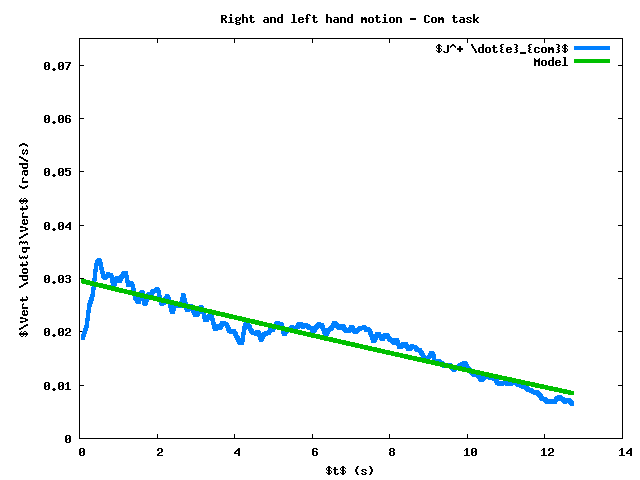
\includegraphics{img/exp1/RL/invJerror_taskCom_0}}%
    \gplfronttext
  \end{picture}%
\endgroup

    }\\
  $r = 0.245544 $ & $r = 0.103142$\\
\end{tabular*}
\caption{Comparison of the fitting for the center of masses regulation task for the \emph{both hands} and \emph{right hand} motion at the first iteration of the identification algorithm.
The residues $r$ of the optimizations are showed in the second row.}
\label{fig:exp1:taskCom0}
\end{figure*}

\begin{figure*}[t]
\begin{tabular*}{0.9\textwidth}{@{\extracolsep{\fill}}cc}
  \resizebox{.4\textwidth}{!} {
	% GNUPLOT: LaTeX picture with Postscript
\begingroup
  \makeatletter
  \providecommand\color[2][]{%
    \GenericError{(gnuplot) \space\space\space\@spaces}{%
      Package color not loaded in conjunction with
      terminal option `colourtext'%
    }{See the gnuplot documentation for explanation.%
    }{Either use 'blacktext' in gnuplot or load the package
      color.sty in LaTeX.}%
    \renewcommand\color[2][]{}%
  }%
  \providecommand\includegraphics[2][]{%
    \GenericError{(gnuplot) \space\space\space\@spaces}{%
      Package graphicx or graphics not loaded%
    }{See the gnuplot documentation for explanation.%
    }{The gnuplot epslatex terminal needs graphicx.sty or graphics.sty.}%
    \renewcommand\includegraphics[2][]{}%
  }%
  \providecommand\rotatebox[2]{#2}%
  \@ifundefined{ifGPcolor}{%
    \newif\ifGPcolor
    \GPcolortrue
  }{}%
  \@ifundefined{ifGPblacktext}{%
    \newif\ifGPblacktext
    \GPblacktexttrue
  }{}%
  % define a \g@addto@macro without @ in the name:
  \let\gplgaddtomacro\g@addto@macro
  % define empty templates for all commands taking text:
  \gdef\gplbacktext{}%
  \gdef\gplfronttext{}%
  \makeatother
  \ifGPblacktext
    % no textcolor at all
    \def\colorrgb#1{}%
    \def\colorgray#1{}%
  \else
    % gray or color?
    \ifGPcolor
      \def\colorrgb#1{\color[rgb]{#1}}%
      \def\colorgray#1{\color[gray]{#1}}%
      \expandafter\def\csname LTw\endcsname{\color{white}}%
      \expandafter\def\csname LTb\endcsname{\color{black}}%
      \expandafter\def\csname LTa\endcsname{\color{black}}%
      \expandafter\def\csname LT0\endcsname{\color[rgb]{1,0,0}}%
      \expandafter\def\csname LT1\endcsname{\color[rgb]{0,1,0}}%
      \expandafter\def\csname LT2\endcsname{\color[rgb]{0,0,1}}%
      \expandafter\def\csname LT3\endcsname{\color[rgb]{1,0,1}}%
      \expandafter\def\csname LT4\endcsname{\color[rgb]{0,1,1}}%
      \expandafter\def\csname LT5\endcsname{\color[rgb]{1,1,0}}%
      \expandafter\def\csname LT6\endcsname{\color[rgb]{0,0,0}}%
      \expandafter\def\csname LT7\endcsname{\color[rgb]{1,0.3,0}}%
      \expandafter\def\csname LT8\endcsname{\color[rgb]{0.5,0.5,0.5}}%
    \else
      % gray
      \def\colorrgb#1{\color{black}}%
      \def\colorgray#1{\color[gray]{#1}}%
      \expandafter\def\csname LTw\endcsname{\color{white}}%
      \expandafter\def\csname LTb\endcsname{\color{black}}%
      \expandafter\def\csname LTa\endcsname{\color{black}}%
      \expandafter\def\csname LT0\endcsname{\color{black}}%
      \expandafter\def\csname LT1\endcsname{\color{black}}%
      \expandafter\def\csname LT2\endcsname{\color{black}}%
      \expandafter\def\csname LT3\endcsname{\color{black}}%
      \expandafter\def\csname LT4\endcsname{\color{black}}%
      \expandafter\def\csname LT5\endcsname{\color{black}}%
      \expandafter\def\csname LT6\endcsname{\color{black}}%
      \expandafter\def\csname LT7\endcsname{\color{black}}%
      \expandafter\def\csname LT8\endcsname{\color{black}}%
    \fi
  \fi
  \setlength{\unitlength}{0.0500bp}%
  \begin{picture}(7200.00,5040.00)%
    \gplgaddtomacro\gplbacktext{%
      \csname LTb\endcsname%
      \put(1210,704){\makebox(0,0)[r]{\strut{} 0}}%
      \put(1210,1229){\makebox(0,0)[r]{\strut{} 0.1}}%
      \put(1210,1754){\makebox(0,0)[r]{\strut{} 0.2}}%
      \put(1210,2279){\makebox(0,0)[r]{\strut{} 0.3}}%
      \put(1210,2805){\makebox(0,0)[r]{\strut{} 0.4}}%
      \put(1210,3330){\makebox(0,0)[r]{\strut{} 0.5}}%
      \put(1210,3855){\makebox(0,0)[r]{\strut{} 0.6}}%
      \put(1210,4380){\makebox(0,0)[r]{\strut{} 0.7}}%
      \put(1342,484){\makebox(0,0){\strut{} 0}}%
      \put(2192,484){\makebox(0,0){\strut{} 2}}%
      \put(3043,484){\makebox(0,0){\strut{} 4}}%
      \put(3893,484){\makebox(0,0){\strut{} 6}}%
      \put(4744,484){\makebox(0,0){\strut{} 8}}%
      \put(5594,484){\makebox(0,0){\strut{} 10}}%
      \put(6445,484){\makebox(0,0){\strut{} 12}}%
      \put(440,2542){\rotatebox{90}{\makebox(0,0){\strut{}$\Vert \dot{q}\Vert$ (rad/s)}}}%
      \put(4106,154){\makebox(0,0){\strut{}$t$ (s)}}%
      \put(4106,4710){\makebox(0,0){\strut{}$\begin{array}{rl} r &= 2.81959\\ \int \Vert J^+ \dot{e}_{head} \Vert \mathrm{d}t &=  0.0355852 \mathrm{rad}\\ \end{array}$}}%
    }%
    \gplgaddtomacro\gplfronttext{%
      \csname LTb\endcsname%
      \put(5883,4207){\makebox(0,0)[r]{\strut{}$J^+ \dot{e}_{head} / \int \Vert J^+ \dot{e}_{head} \Vert \mathrm{d}t$}}%
      \csname LTb\endcsname%
      \put(5883,3987){\makebox(0,0)[r]{\strut{}Model}}%
    }%
    \gplbacktext
    \put(0,0){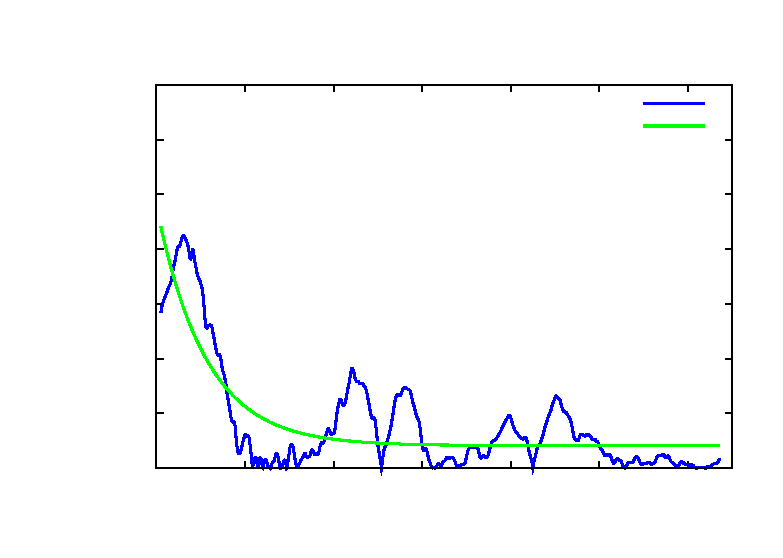
\includegraphics{img/exp1/R/invJerror_taskHead_0}}%
    \gplfronttext
  \end{picture}%
\endgroup

    }                           &
  \resizebox{.4\textwidth}{!} {
	% GNUPLOT: LaTeX picture with Postscript
\begingroup
  \makeatletter
  \providecommand\color[2][]{%
    \GenericError{(gnuplot) \space\space\space\@spaces}{%
      Package color not loaded in conjunction with
      terminal option `colourtext'%
    }{See the gnuplot documentation for explanation.%
    }{Either use 'blacktext' in gnuplot or load the package
      color.sty in LaTeX.}%
    \renewcommand\color[2][]{}%
  }%
  \providecommand\includegraphics[2][]{%
    \GenericError{(gnuplot) \space\space\space\@spaces}{%
      Package graphicx or graphics not loaded%
    }{See the gnuplot documentation for explanation.%
    }{The gnuplot epslatex terminal needs graphicx.sty or graphics.sty.}%
    \renewcommand\includegraphics[2][]{}%
  }%
  \providecommand\rotatebox[2]{#2}%
  \@ifundefined{ifGPcolor}{%
    \newif\ifGPcolor
    \GPcolortrue
  }{}%
  \@ifundefined{ifGPblacktext}{%
    \newif\ifGPblacktext
    \GPblacktexttrue
  }{}%
  % define a \g@addto@macro without @ in the name:
  \let\gplgaddtomacro\g@addto@macro
  % define empty templates for all commands taking text:
  \gdef\gplbacktext{}%
  \gdef\gplfronttext{}%
  \makeatother
  \ifGPblacktext
    % no textcolor at all
    \def\colorrgb#1{}%
    \def\colorgray#1{}%
  \else
    % gray or color?
    \ifGPcolor
      \def\colorrgb#1{\color[rgb]{#1}}%
      \def\colorgray#1{\color[gray]{#1}}%
      \expandafter\def\csname LTw\endcsname{\color{white}}%
      \expandafter\def\csname LTb\endcsname{\color{black}}%
      \expandafter\def\csname LTa\endcsname{\color{black}}%
      \expandafter\def\csname LT0\endcsname{\color[rgb]{1,0,0}}%
      \expandafter\def\csname LT1\endcsname{\color[rgb]{0,1,0}}%
      \expandafter\def\csname LT2\endcsname{\color[rgb]{0,0,1}}%
      \expandafter\def\csname LT3\endcsname{\color[rgb]{1,0,1}}%
      \expandafter\def\csname LT4\endcsname{\color[rgb]{0,1,1}}%
      \expandafter\def\csname LT5\endcsname{\color[rgb]{1,1,0}}%
      \expandafter\def\csname LT6\endcsname{\color[rgb]{0,0,0}}%
      \expandafter\def\csname LT7\endcsname{\color[rgb]{1,0.3,0}}%
      \expandafter\def\csname LT8\endcsname{\color[rgb]{0.5,0.5,0.5}}%
    \else
      % gray
      \def\colorrgb#1{\color{black}}%
      \def\colorgray#1{\color[gray]{#1}}%
      \expandafter\def\csname LTw\endcsname{\color{white}}%
      \expandafter\def\csname LTb\endcsname{\color{black}}%
      \expandafter\def\csname LTa\endcsname{\color{black}}%
      \expandafter\def\csname LT0\endcsname{\color{black}}%
      \expandafter\def\csname LT1\endcsname{\color{black}}%
      \expandafter\def\csname LT2\endcsname{\color{black}}%
      \expandafter\def\csname LT3\endcsname{\color{black}}%
      \expandafter\def\csname LT4\endcsname{\color{black}}%
      \expandafter\def\csname LT5\endcsname{\color{black}}%
      \expandafter\def\csname LT6\endcsname{\color{black}}%
      \expandafter\def\csname LT7\endcsname{\color{black}}%
      \expandafter\def\csname LT8\endcsname{\color{black}}%
    \fi
  \fi
  \setlength{\unitlength}{0.0500bp}%
  \begin{picture}(7200.00,5040.00)%
    \gplgaddtomacro\gplbacktext{%
      \csname LTb\endcsname%
      \put(1342,704){\makebox(0,0)[r]{\strut{} 0}}%
      \put(1342,1194){\makebox(0,0)[r]{\strut{} 0.01}}%
      \put(1342,1684){\makebox(0,0)[r]{\strut{} 0.02}}%
      \put(1342,2174){\makebox(0,0)[r]{\strut{} 0.03}}%
      \put(1342,2665){\makebox(0,0)[r]{\strut{} 0.04}}%
      \put(1342,3155){\makebox(0,0)[r]{\strut{} 0.05}}%
      \put(1342,3645){\makebox(0,0)[r]{\strut{} 0.06}}%
      \put(1342,4135){\makebox(0,0)[r]{\strut{} 0.07}}%
      \put(1474,484){\makebox(0,0){\strut{} 0}}%
      \put(2245,484){\makebox(0,0){\strut{} 2}}%
      \put(3016,484){\makebox(0,0){\strut{} 4}}%
      \put(3787,484){\makebox(0,0){\strut{} 6}}%
      \put(4557,484){\makebox(0,0){\strut{} 8}}%
      \put(5328,484){\makebox(0,0){\strut{} 10}}%
      \put(6099,484){\makebox(0,0){\strut{} 12}}%
      \put(6870,484){\makebox(0,0){\strut{} 14}}%
      \put(440,2542){\rotatebox{90}{\makebox(0,0){\strut{}$\Vert \dot{q}\Vert$ (rad/s)}}}%
      \put(4172,154){\makebox(0,0){\strut{}$t$ (s)}}%
      \put(4172,4710){\makebox(0,0){\strut{}Right and left hand motion - Head task}}%
    }%
    \gplgaddtomacro\gplfronttext{%
      \csname LTb\endcsname%
      \put(5883,4207){\makebox(0,0)[r]{\strut{}$J^+ \dot{e}_{head}$}}%
      \csname LTb\endcsname%
      \put(5883,3987){\makebox(0,0)[r]{\strut{}Model}}%
    }%
    \gplbacktext
    \put(0,0){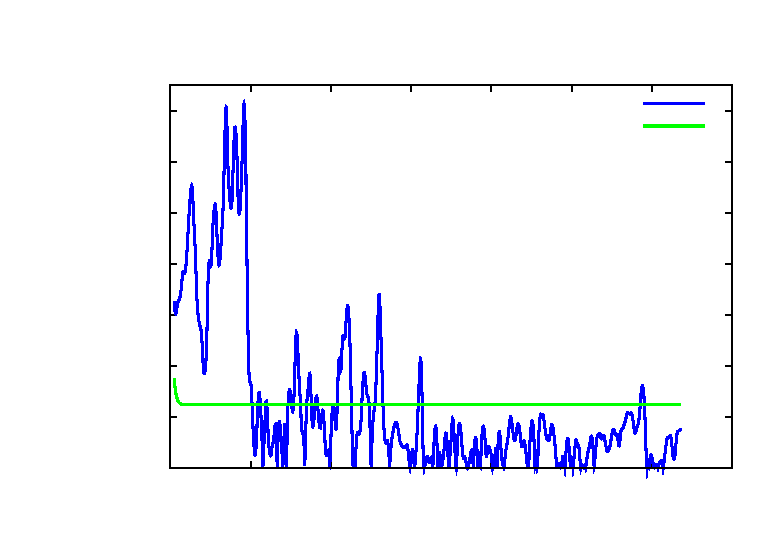
\includegraphics{img/exp1/RL/invJerror_taskHead_0}}%
    \gplfronttext
  \end{picture}%
\endgroup

    }\\
  $r = 0.439323 $ & $r = 0.771167$\\
\end{tabular*}
\caption{Comparison of the fitting for the head task for the \emph{both hands} and \emph{right hand} motion at the first iteration of the identification algorithm.
The residues $r$ of the optimizations are showed in the second row.}
\label{fig:exp1:taskHead0}
\end{figure*}

\begin{figure*}[t]
\begin{tabular*}{0.9\textwidth}{@{\extracolsep{\fill}}cc}
  \resizebox{.4\textwidth}{!} {
	% GNUPLOT: LaTeX picture with Postscript
\begingroup
  \makeatletter
  \providecommand\color[2][]{%
    \GenericError{(gnuplot) \space\space\space\@spaces}{%
      Package color not loaded in conjunction with
      terminal option `colourtext'%
    }{See the gnuplot documentation for explanation.%
    }{Either use 'blacktext' in gnuplot or load the package
      color.sty in LaTeX.}%
    \renewcommand\color[2][]{}%
  }%
  \providecommand\includegraphics[2][]{%
    \GenericError{(gnuplot) \space\space\space\@spaces}{%
      Package graphicx or graphics not loaded%
    }{See the gnuplot documentation for explanation.%
    }{The gnuplot epslatex terminal needs graphicx.sty or graphics.sty.}%
    \renewcommand\includegraphics[2][]{}%
  }%
  \providecommand\rotatebox[2]{#2}%
  \@ifundefined{ifGPcolor}{%
    \newif\ifGPcolor
    \GPcolortrue
  }{}%
  \@ifundefined{ifGPblacktext}{%
    \newif\ifGPblacktext
    \GPblacktexttrue
  }{}%
  % define a \g@addto@macro without @ in the name:
  \let\gplgaddtomacro\g@addto@macro
  % define empty templates for all commands taking text:
  \gdef\gplbacktext{}%
  \gdef\gplfronttext{}%
  \makeatother
  \ifGPblacktext
    % no textcolor at all
    \def\colorrgb#1{}%
    \def\colorgray#1{}%
  \else
    % gray or color?
    \ifGPcolor
      \def\colorrgb#1{\color[rgb]{#1}}%
      \def\colorgray#1{\color[gray]{#1}}%
      \expandafter\def\csname LTw\endcsname{\color{white}}%
      \expandafter\def\csname LTb\endcsname{\color{black}}%
      \expandafter\def\csname LTa\endcsname{\color{black}}%
      \expandafter\def\csname LT0\endcsname{\color[rgb]{1,0,0}}%
      \expandafter\def\csname LT1\endcsname{\color[rgb]{0,1,0}}%
      \expandafter\def\csname LT2\endcsname{\color[rgb]{0,0,1}}%
      \expandafter\def\csname LT3\endcsname{\color[rgb]{1,0,1}}%
      \expandafter\def\csname LT4\endcsname{\color[rgb]{0,1,1}}%
      \expandafter\def\csname LT5\endcsname{\color[rgb]{1,1,0}}%
      \expandafter\def\csname LT6\endcsname{\color[rgb]{0,0,0}}%
      \expandafter\def\csname LT7\endcsname{\color[rgb]{1,0.3,0}}%
      \expandafter\def\csname LT8\endcsname{\color[rgb]{0.5,0.5,0.5}}%
    \else
      % gray
      \def\colorrgb#1{\color{black}}%
      \def\colorgray#1{\color[gray]{#1}}%
      \expandafter\def\csname LTw\endcsname{\color{white}}%
      \expandafter\def\csname LTb\endcsname{\color{black}}%
      \expandafter\def\csname LTa\endcsname{\color{black}}%
      \expandafter\def\csname LT0\endcsname{\color{black}}%
      \expandafter\def\csname LT1\endcsname{\color{black}}%
      \expandafter\def\csname LT2\endcsname{\color{black}}%
      \expandafter\def\csname LT3\endcsname{\color{black}}%
      \expandafter\def\csname LT4\endcsname{\color{black}}%
      \expandafter\def\csname LT5\endcsname{\color{black}}%
      \expandafter\def\csname LT6\endcsname{\color{black}}%
      \expandafter\def\csname LT7\endcsname{\color{black}}%
      \expandafter\def\csname LT8\endcsname{\color{black}}%
    \fi
  \fi
  \setlength{\unitlength}{0.0500bp}%
  \begin{picture}(7200.00,5040.00)%
    \gplgaddtomacro\gplbacktext{%
      \csname LTb\endcsname%
      \put(1342,704){\makebox(0,0)[r]{\strut{} 0}}%
      \put(1342,1194){\makebox(0,0)[r]{\strut{} 0.01}}%
      \put(1342,1684){\makebox(0,0)[r]{\strut{} 0.02}}%
      \put(1342,2174){\makebox(0,0)[r]{\strut{} 0.03}}%
      \put(1342,2665){\makebox(0,0)[r]{\strut{} 0.04}}%
      \put(1342,3155){\makebox(0,0)[r]{\strut{} 0.05}}%
      \put(1342,3645){\makebox(0,0)[r]{\strut{} 0.06}}%
      \put(1342,4135){\makebox(0,0)[r]{\strut{} 0.07}}%
      \put(1474,484){\makebox(0,0){\strut{} 0}}%
      \put(2245,484){\makebox(0,0){\strut{} 2}}%
      \put(3016,484){\makebox(0,0){\strut{} 4}}%
      \put(3787,484){\makebox(0,0){\strut{} 6}}%
      \put(4557,484){\makebox(0,0){\strut{} 8}}%
      \put(5328,484){\makebox(0,0){\strut{} 10}}%
      \put(6099,484){\makebox(0,0){\strut{} 12}}%
      \put(6870,484){\makebox(0,0){\strut{} 14}}%
      \put(440,2542){\rotatebox{90}{\makebox(0,0){\strut{}$\Vert \dot{q}\Vert$ (rad/s)}}}%
      \put(4172,154){\makebox(0,0){\strut{}$t$ (s)}}%
      \put(4172,4710){\makebox(0,0){\strut{}Right hand motion - Left Hand task}}%
    }%
    \gplgaddtomacro\gplfronttext{%
      \csname LTb\endcsname%
      \put(5883,4207){\makebox(0,0)[r]{\strut{}$J^+ \dot{e}_{lhand}$}}%
      \csname LTb\endcsname%
      \put(5883,3987){\makebox(0,0)[r]{\strut{}Model}}%
    }%
    \gplbacktext
    \put(0,0){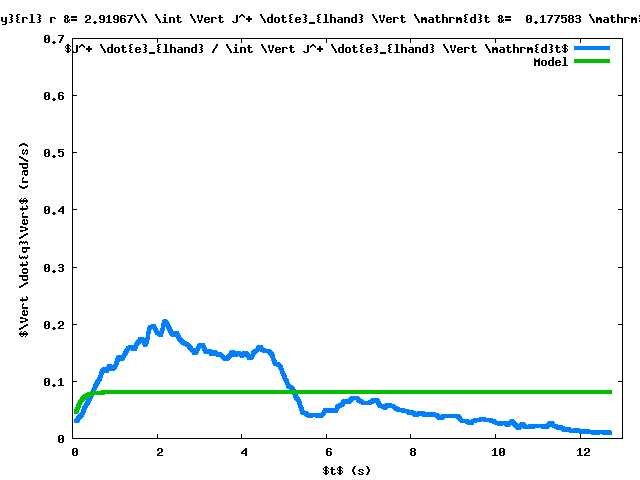
\includegraphics{img/exp1/R/invJerror_taskLhand_0}}%
    \gplfronttext
  \end{picture}%
\endgroup

    }                           &
  \resizebox{.4\textwidth}{!} {
	% GNUPLOT: LaTeX picture with Postscript
\begingroup
  \makeatletter
  \providecommand\color[2][]{%
    \GenericError{(gnuplot) \space\space\space\@spaces}{%
      Package color not loaded in conjunction with
      terminal option `colourtext'%
    }{See the gnuplot documentation for explanation.%
    }{Either use 'blacktext' in gnuplot or load the package
      color.sty in LaTeX.}%
    \renewcommand\color[2][]{}%
  }%
  \providecommand\includegraphics[2][]{%
    \GenericError{(gnuplot) \space\space\space\@spaces}{%
      Package graphicx or graphics not loaded%
    }{See the gnuplot documentation for explanation.%
    }{The gnuplot epslatex terminal needs graphicx.sty or graphics.sty.}%
    \renewcommand\includegraphics[2][]{}%
  }%
  \providecommand\rotatebox[2]{#2}%
  \@ifundefined{ifGPcolor}{%
    \newif\ifGPcolor
    \GPcolortrue
  }{}%
  \@ifundefined{ifGPblacktext}{%
    \newif\ifGPblacktext
    \GPblacktexttrue
  }{}%
  % define a \g@addto@macro without @ in the name:
  \let\gplgaddtomacro\g@addto@macro
  % define empty templates for all commands taking text:
  \gdef\gplbacktext{}%
  \gdef\gplfronttext{}%
  \makeatother
  \ifGPblacktext
    % no textcolor at all
    \def\colorrgb#1{}%
    \def\colorgray#1{}%
  \else
    % gray or color?
    \ifGPcolor
      \def\colorrgb#1{\color[rgb]{#1}}%
      \def\colorgray#1{\color[gray]{#1}}%
      \expandafter\def\csname LTw\endcsname{\color{white}}%
      \expandafter\def\csname LTb\endcsname{\color{black}}%
      \expandafter\def\csname LTa\endcsname{\color{black}}%
      \expandafter\def\csname LT0\endcsname{\color[rgb]{1,0,0}}%
      \expandafter\def\csname LT1\endcsname{\color[rgb]{0,1,0}}%
      \expandafter\def\csname LT2\endcsname{\color[rgb]{0,0,1}}%
      \expandafter\def\csname LT3\endcsname{\color[rgb]{1,0,1}}%
      \expandafter\def\csname LT4\endcsname{\color[rgb]{0,1,1}}%
      \expandafter\def\csname LT5\endcsname{\color[rgb]{1,1,0}}%
      \expandafter\def\csname LT6\endcsname{\color[rgb]{0,0,0}}%
      \expandafter\def\csname LT7\endcsname{\color[rgb]{1,0.3,0}}%
      \expandafter\def\csname LT8\endcsname{\color[rgb]{0.5,0.5,0.5}}%
    \else
      % gray
      \def\colorrgb#1{\color{black}}%
      \def\colorgray#1{\color[gray]{#1}}%
      \expandafter\def\csname LTw\endcsname{\color{white}}%
      \expandafter\def\csname LTb\endcsname{\color{black}}%
      \expandafter\def\csname LTa\endcsname{\color{black}}%
      \expandafter\def\csname LT0\endcsname{\color{black}}%
      \expandafter\def\csname LT1\endcsname{\color{black}}%
      \expandafter\def\csname LT2\endcsname{\color{black}}%
      \expandafter\def\csname LT3\endcsname{\color{black}}%
      \expandafter\def\csname LT4\endcsname{\color{black}}%
      \expandafter\def\csname LT5\endcsname{\color{black}}%
      \expandafter\def\csname LT6\endcsname{\color{black}}%
      \expandafter\def\csname LT7\endcsname{\color{black}}%
      \expandafter\def\csname LT8\endcsname{\color{black}}%
    \fi
  \fi
  \setlength{\unitlength}{0.0500bp}%
  \begin{picture}(7200.00,5040.00)%
    \gplgaddtomacro\gplbacktext{%
      \csname LTb\endcsname%
      \put(1342,704){\makebox(0,0)[r]{\strut{} 0}}%
      \put(1342,1194){\makebox(0,0)[r]{\strut{} 0.01}}%
      \put(1342,1684){\makebox(0,0)[r]{\strut{} 0.02}}%
      \put(1342,2174){\makebox(0,0)[r]{\strut{} 0.03}}%
      \put(1342,2665){\makebox(0,0)[r]{\strut{} 0.04}}%
      \put(1342,3155){\makebox(0,0)[r]{\strut{} 0.05}}%
      \put(1342,3645){\makebox(0,0)[r]{\strut{} 0.06}}%
      \put(1342,4135){\makebox(0,0)[r]{\strut{} 0.07}}%
      \put(1474,484){\makebox(0,0){\strut{} 0}}%
      \put(2245,484){\makebox(0,0){\strut{} 2}}%
      \put(3016,484){\makebox(0,0){\strut{} 4}}%
      \put(3787,484){\makebox(0,0){\strut{} 6}}%
      \put(4557,484){\makebox(0,0){\strut{} 8}}%
      \put(5328,484){\makebox(0,0){\strut{} 10}}%
      \put(6099,484){\makebox(0,0){\strut{} 12}}%
      \put(6870,484){\makebox(0,0){\strut{} 14}}%
      \put(440,2542){\rotatebox{90}{\makebox(0,0){\strut{}$\Vert \dot{q}\Vert$ (rad/s)}}}%
      \put(4172,154){\makebox(0,0){\strut{}$t$ (s)}}%
      \put(4172,4710){\makebox(0,0){\strut{}Right and left hand motion - Left hand task}}%
    }%
    \gplgaddtomacro\gplfronttext{%
      \csname LTb\endcsname%
      \put(5883,4207){\makebox(0,0)[r]{\strut{}$J^+ \dot{e}_{lhand}$}}%
      \csname LTb\endcsname%
      \put(5883,3987){\makebox(0,0)[r]{\strut{}Model}}%
    }%
    \gplbacktext
    \put(0,0){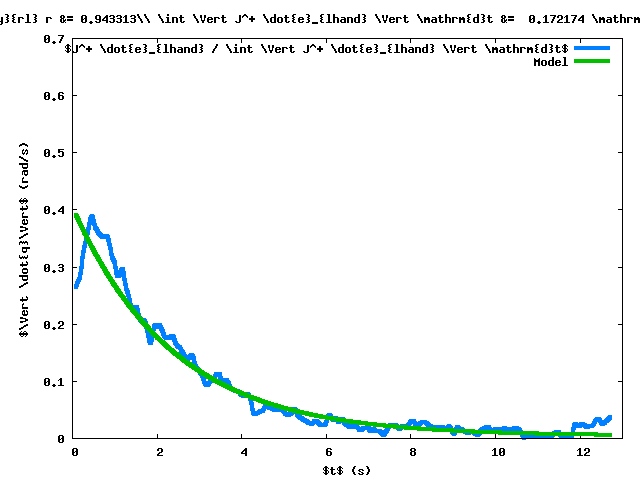
\includegraphics{img/exp1/RL/invJerror_taskLhand_0}}%
    \gplfronttext
  \end{picture}%
\endgroup

    }\\
  $r = 0.590588 $ & $r = 0.147667$\\
\end{tabular*}
\caption{Comparison of the fitting for the left hand task for the \emph{both hands} and \emph{right hand} motion at the first iteration of the identification algorithm.
The residues $r$ of the optimizations are showed in the second row.}
\label{fig:exp1:taskLhand00}
\end{figure*}

\begin{figure*}[t]
\begin{tabular*}{0.9\textwidth}{@{\extracolsep{\fill}}cc}
  \resizebox{.4\textwidth}{!} {
	% GNUPLOT: LaTeX picture with Postscript
\begingroup
  \makeatletter
  \providecommand\color[2][]{%
    \GenericError{(gnuplot) \space\space\space\@spaces}{%
      Package color not loaded in conjunction with
      terminal option `colourtext'%
    }{See the gnuplot documentation for explanation.%
    }{Either use 'blacktext' in gnuplot or load the package
      color.sty in LaTeX.}%
    \renewcommand\color[2][]{}%
  }%
  \providecommand\includegraphics[2][]{%
    \GenericError{(gnuplot) \space\space\space\@spaces}{%
      Package graphicx or graphics not loaded%
    }{See the gnuplot documentation for explanation.%
    }{The gnuplot epslatex terminal needs graphicx.sty or graphics.sty.}%
    \renewcommand\includegraphics[2][]{}%
  }%
  \providecommand\rotatebox[2]{#2}%
  \@ifundefined{ifGPcolor}{%
    \newif\ifGPcolor
    \GPcolortrue
  }{}%
  \@ifundefined{ifGPblacktext}{%
    \newif\ifGPblacktext
    \GPblacktexttrue
  }{}%
  % define a \g@addto@macro without @ in the name:
  \let\gplgaddtomacro\g@addto@macro
  % define empty templates for all commands taking text:
  \gdef\gplbacktext{}%
  \gdef\gplfronttext{}%
  \makeatother
  \ifGPblacktext
    % no textcolor at all
    \def\colorrgb#1{}%
    \def\colorgray#1{}%
  \else
    % gray or color?
    \ifGPcolor
      \def\colorrgb#1{\color[rgb]{#1}}%
      \def\colorgray#1{\color[gray]{#1}}%
      \expandafter\def\csname LTw\endcsname{\color{white}}%
      \expandafter\def\csname LTb\endcsname{\color{black}}%
      \expandafter\def\csname LTa\endcsname{\color{black}}%
      \expandafter\def\csname LT0\endcsname{\color[rgb]{1,0,0}}%
      \expandafter\def\csname LT1\endcsname{\color[rgb]{0,1,0}}%
      \expandafter\def\csname LT2\endcsname{\color[rgb]{0,0,1}}%
      \expandafter\def\csname LT3\endcsname{\color[rgb]{1,0,1}}%
      \expandafter\def\csname LT4\endcsname{\color[rgb]{0,1,1}}%
      \expandafter\def\csname LT5\endcsname{\color[rgb]{1,1,0}}%
      \expandafter\def\csname LT6\endcsname{\color[rgb]{0,0,0}}%
      \expandafter\def\csname LT7\endcsname{\color[rgb]{1,0.3,0}}%
      \expandafter\def\csname LT8\endcsname{\color[rgb]{0.5,0.5,0.5}}%
    \else
      % gray
      \def\colorrgb#1{\color{black}}%
      \def\colorgray#1{\color[gray]{#1}}%
      \expandafter\def\csname LTw\endcsname{\color{white}}%
      \expandafter\def\csname LTb\endcsname{\color{black}}%
      \expandafter\def\csname LTa\endcsname{\color{black}}%
      \expandafter\def\csname LT0\endcsname{\color{black}}%
      \expandafter\def\csname LT1\endcsname{\color{black}}%
      \expandafter\def\csname LT2\endcsname{\color{black}}%
      \expandafter\def\csname LT3\endcsname{\color{black}}%
      \expandafter\def\csname LT4\endcsname{\color{black}}%
      \expandafter\def\csname LT5\endcsname{\color{black}}%
      \expandafter\def\csname LT6\endcsname{\color{black}}%
      \expandafter\def\csname LT7\endcsname{\color{black}}%
      \expandafter\def\csname LT8\endcsname{\color{black}}%
    \fi
  \fi
  \setlength{\unitlength}{0.0500bp}%
  \begin{picture}(7200.00,5040.00)%
    \gplgaddtomacro\gplbacktext{%
      \csname LTb\endcsname%
      \put(1342,704){\makebox(0,0)[r]{\strut{} 0}}%
      \put(1342,1194){\makebox(0,0)[r]{\strut{} 0.01}}%
      \put(1342,1684){\makebox(0,0)[r]{\strut{} 0.02}}%
      \put(1342,2174){\makebox(0,0)[r]{\strut{} 0.03}}%
      \put(1342,2665){\makebox(0,0)[r]{\strut{} 0.04}}%
      \put(1342,3155){\makebox(0,0)[r]{\strut{} 0.05}}%
      \put(1342,3645){\makebox(0,0)[r]{\strut{} 0.06}}%
      \put(1342,4135){\makebox(0,0)[r]{\strut{} 0.07}}%
      \put(1474,484){\makebox(0,0){\strut{} 0}}%
      \put(2245,484){\makebox(0,0){\strut{} 2}}%
      \put(3016,484){\makebox(0,0){\strut{} 4}}%
      \put(3787,484){\makebox(0,0){\strut{} 6}}%
      \put(4557,484){\makebox(0,0){\strut{} 8}}%
      \put(5328,484){\makebox(0,0){\strut{} 10}}%
      \put(6099,484){\makebox(0,0){\strut{} 12}}%
      \put(6870,484){\makebox(0,0){\strut{} 14}}%
      \put(440,2542){\rotatebox{90}{\makebox(0,0){\strut{}$\Vert \dot{q}\Vert$ (rad/s)}}}%
      \put(4172,154){\makebox(0,0){\strut{}$t$ (s)}}%
      \put(4172,4710){\makebox(0,0){\strut{}Right hand motion - Right Hand task}}%
    }%
    \gplgaddtomacro\gplfronttext{%
      \csname LTb\endcsname%
      \put(5883,4207){\makebox(0,0)[r]{\strut{}$J^+ \dot{e}_{rhand}$}}%
      \csname LTb\endcsname%
      \put(5883,3987){\makebox(0,0)[r]{\strut{}Model}}%
    }%
    \gplbacktext
    \put(0,0){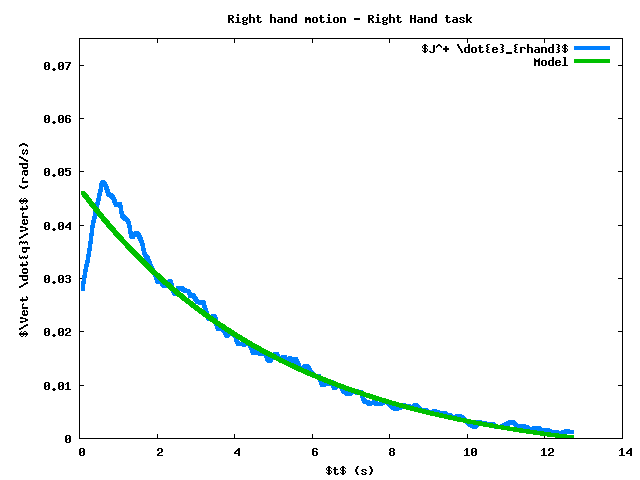
\includegraphics{img/exp1/R/invJerror_taskRhand_0}}%
    \gplfronttext
  \end{picture}%
\endgroup

    }                           &
  \resizebox{.4\textwidth}{!} {
	% GNUPLOT: LaTeX picture with Postscript
\begingroup
  \makeatletter
  \providecommand\color[2][]{%
    \GenericError{(gnuplot) \space\space\space\@spaces}{%
      Package color not loaded in conjunction with
      terminal option `colourtext'%
    }{See the gnuplot documentation for explanation.%
    }{Either use 'blacktext' in gnuplot or load the package
      color.sty in LaTeX.}%
    \renewcommand\color[2][]{}%
  }%
  \providecommand\includegraphics[2][]{%
    \GenericError{(gnuplot) \space\space\space\@spaces}{%
      Package graphicx or graphics not loaded%
    }{See the gnuplot documentation for explanation.%
    }{The gnuplot epslatex terminal needs graphicx.sty or graphics.sty.}%
    \renewcommand\includegraphics[2][]{}%
  }%
  \providecommand\rotatebox[2]{#2}%
  \@ifundefined{ifGPcolor}{%
    \newif\ifGPcolor
    \GPcolortrue
  }{}%
  \@ifundefined{ifGPblacktext}{%
    \newif\ifGPblacktext
    \GPblacktexttrue
  }{}%
  % define a \g@addto@macro without @ in the name:
  \let\gplgaddtomacro\g@addto@macro
  % define empty templates for all commands taking text:
  \gdef\gplbacktext{}%
  \gdef\gplfronttext{}%
  \makeatother
  \ifGPblacktext
    % no textcolor at all
    \def\colorrgb#1{}%
    \def\colorgray#1{}%
  \else
    % gray or color?
    \ifGPcolor
      \def\colorrgb#1{\color[rgb]{#1}}%
      \def\colorgray#1{\color[gray]{#1}}%
      \expandafter\def\csname LTw\endcsname{\color{white}}%
      \expandafter\def\csname LTb\endcsname{\color{black}}%
      \expandafter\def\csname LTa\endcsname{\color{black}}%
      \expandafter\def\csname LT0\endcsname{\color[rgb]{1,0,0}}%
      \expandafter\def\csname LT1\endcsname{\color[rgb]{0,1,0}}%
      \expandafter\def\csname LT2\endcsname{\color[rgb]{0,0,1}}%
      \expandafter\def\csname LT3\endcsname{\color[rgb]{1,0,1}}%
      \expandafter\def\csname LT4\endcsname{\color[rgb]{0,1,1}}%
      \expandafter\def\csname LT5\endcsname{\color[rgb]{1,1,0}}%
      \expandafter\def\csname LT6\endcsname{\color[rgb]{0,0,0}}%
      \expandafter\def\csname LT7\endcsname{\color[rgb]{1,0.3,0}}%
      \expandafter\def\csname LT8\endcsname{\color[rgb]{0.5,0.5,0.5}}%
    \else
      % gray
      \def\colorrgb#1{\color{black}}%
      \def\colorgray#1{\color[gray]{#1}}%
      \expandafter\def\csname LTw\endcsname{\color{white}}%
      \expandafter\def\csname LTb\endcsname{\color{black}}%
      \expandafter\def\csname LTa\endcsname{\color{black}}%
      \expandafter\def\csname LT0\endcsname{\color{black}}%
      \expandafter\def\csname LT1\endcsname{\color{black}}%
      \expandafter\def\csname LT2\endcsname{\color{black}}%
      \expandafter\def\csname LT3\endcsname{\color{black}}%
      \expandafter\def\csname LT4\endcsname{\color{black}}%
      \expandafter\def\csname LT5\endcsname{\color{black}}%
      \expandafter\def\csname LT6\endcsname{\color{black}}%
      \expandafter\def\csname LT7\endcsname{\color{black}}%
      \expandafter\def\csname LT8\endcsname{\color{black}}%
    \fi
  \fi
  \setlength{\unitlength}{0.0500bp}%
  \begin{picture}(7200.00,5040.00)%
    \gplgaddtomacro\gplbacktext{%
      \csname LTb\endcsname%
      \put(1210,704){\makebox(0,0)[r]{\strut{} 0}}%
      \put(1210,1229){\makebox(0,0)[r]{\strut{} 0.1}}%
      \put(1210,1754){\makebox(0,0)[r]{\strut{} 0.2}}%
      \put(1210,2279){\makebox(0,0)[r]{\strut{} 0.3}}%
      \put(1210,2805){\makebox(0,0)[r]{\strut{} 0.4}}%
      \put(1210,3330){\makebox(0,0)[r]{\strut{} 0.5}}%
      \put(1210,3855){\makebox(0,0)[r]{\strut{} 0.6}}%
      \put(1210,4380){\makebox(0,0)[r]{\strut{} 0.7}}%
      \put(1342,484){\makebox(0,0){\strut{} 0}}%
      \put(2192,484){\makebox(0,0){\strut{} 2}}%
      \put(3043,484){\makebox(0,0){\strut{} 4}}%
      \put(3893,484){\makebox(0,0){\strut{} 6}}%
      \put(4744,484){\makebox(0,0){\strut{} 8}}%
      \put(5594,484){\makebox(0,0){\strut{} 10}}%
      \put(6445,484){\makebox(0,0){\strut{} 12}}%
      \put(440,2542){\rotatebox{90}{\makebox(0,0){\strut{}$\Vert \dot{q}\Vert$ (rad/s)}}}%
      \put(4106,154){\makebox(0,0){\strut{}$t$ (s)}}%
      \put(4106,4710){\makebox(0,0){\strut{}$\begin{array}{rl} r &= 0.47739\\ \int \Vert J^+ \dot{e}_{rhand} \Vert \mathrm{d}t &=  0.356896 \mathrm{rad}\\ \end{array}$}}%
    }%
    \gplgaddtomacro\gplfronttext{%
      \csname LTb\endcsname%
      \put(5883,4207){\makebox(0,0)[r]{\strut{}$J^+ \dot{e}_{rhand} / \int \Vert J^+ \dot{e}_{rhand} \Vert \mathrm{d}t$}}%
      \csname LTb\endcsname%
      \put(5883,3987){\makebox(0,0)[r]{\strut{}Model}}%
    }%
    \gplbacktext
    \put(0,0){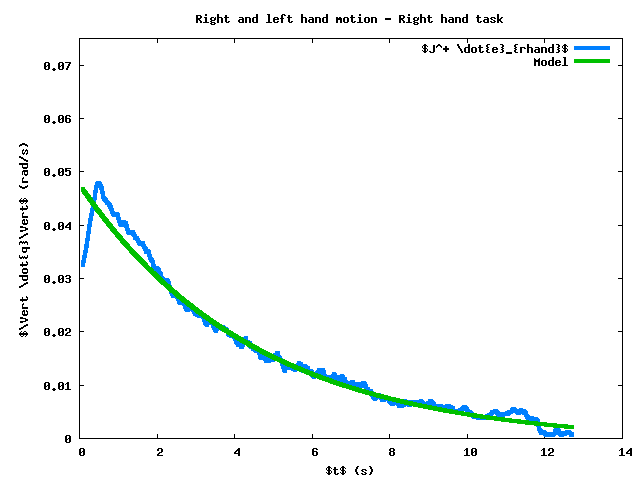
\includegraphics{img/exp1/RL/invJerror_taskRhand_0}}%
    \gplfronttext
  \end{picture}%
\endgroup

    }\\
  $r = 0.11796 $ & $r = 0.0931476$\\
\end{tabular*}
\caption{Comparison of the fitting for the right hand task for the \emph{both hands} and \emph{right hand} motion at the first iteration of the identification algorithm.
The residues $r$ of the optimizations are showed in the second row.}
\label{fig:exp1:taskRhand0}
\end{figure*}

\begin{figure*}[t]
\begin{tabular*}{0.9\textwidth}{@{\extracolsep{\fill}}cc}
  \resizebox{.4\textwidth}{!} {
	% GNUPLOT: LaTeX picture with Postscript
\begingroup
  \makeatletter
  \providecommand\color[2][]{%
    \GenericError{(gnuplot) \space\space\space\@spaces}{%
      Package color not loaded in conjunction with
      terminal option `colourtext'%
    }{See the gnuplot documentation for explanation.%
    }{Either use 'blacktext' in gnuplot or load the package
      color.sty in LaTeX.}%
    \renewcommand\color[2][]{}%
  }%
  \providecommand\includegraphics[2][]{%
    \GenericError{(gnuplot) \space\space\space\@spaces}{%
      Package graphicx or graphics not loaded%
    }{See the gnuplot documentation for explanation.%
    }{The gnuplot epslatex terminal needs graphicx.sty or graphics.sty.}%
    \renewcommand\includegraphics[2][]{}%
  }%
  \providecommand\rotatebox[2]{#2}%
  \@ifundefined{ifGPcolor}{%
    \newif\ifGPcolor
    \GPcolortrue
  }{}%
  \@ifundefined{ifGPblacktext}{%
    \newif\ifGPblacktext
    \GPblacktexttrue
  }{}%
  % define a \g@addto@macro without @ in the name:
  \let\gplgaddtomacro\g@addto@macro
  % define empty templates for all commands taking text:
  \gdef\gplbacktext{}%
  \gdef\gplfronttext{}%
  \makeatother
  \ifGPblacktext
    % no textcolor at all
    \def\colorrgb#1{}%
    \def\colorgray#1{}%
  \else
    % gray or color?
    \ifGPcolor
      \def\colorrgb#1{\color[rgb]{#1}}%
      \def\colorgray#1{\color[gray]{#1}}%
      \expandafter\def\csname LTw\endcsname{\color{white}}%
      \expandafter\def\csname LTb\endcsname{\color{black}}%
      \expandafter\def\csname LTa\endcsname{\color{black}}%
      \expandafter\def\csname LT0\endcsname{\color[rgb]{1,0,0}}%
      \expandafter\def\csname LT1\endcsname{\color[rgb]{0,1,0}}%
      \expandafter\def\csname LT2\endcsname{\color[rgb]{0,0,1}}%
      \expandafter\def\csname LT3\endcsname{\color[rgb]{1,0,1}}%
      \expandafter\def\csname LT4\endcsname{\color[rgb]{0,1,1}}%
      \expandafter\def\csname LT5\endcsname{\color[rgb]{1,1,0}}%
      \expandafter\def\csname LT6\endcsname{\color[rgb]{0,0,0}}%
      \expandafter\def\csname LT7\endcsname{\color[rgb]{1,0.3,0}}%
      \expandafter\def\csname LT8\endcsname{\color[rgb]{0.5,0.5,0.5}}%
    \else
      % gray
      \def\colorrgb#1{\color{black}}%
      \def\colorgray#1{\color[gray]{#1}}%
      \expandafter\def\csname LTw\endcsname{\color{white}}%
      \expandafter\def\csname LTb\endcsname{\color{black}}%
      \expandafter\def\csname LTa\endcsname{\color{black}}%
      \expandafter\def\csname LT0\endcsname{\color{black}}%
      \expandafter\def\csname LT1\endcsname{\color{black}}%
      \expandafter\def\csname LT2\endcsname{\color{black}}%
      \expandafter\def\csname LT3\endcsname{\color{black}}%
      \expandafter\def\csname LT4\endcsname{\color{black}}%
      \expandafter\def\csname LT5\endcsname{\color{black}}%
      \expandafter\def\csname LT6\endcsname{\color{black}}%
      \expandafter\def\csname LT7\endcsname{\color{black}}%
      \expandafter\def\csname LT8\endcsname{\color{black}}%
    \fi
  \fi
  \setlength{\unitlength}{0.0500bp}%
  \begin{picture}(7200.00,5040.00)%
    \gplgaddtomacro\gplbacktext{%
      \csname LTb\endcsname%
      \put(1342,704){\makebox(0,0)[r]{\strut{} 0}}%
      \put(1342,1194){\makebox(0,0)[r]{\strut{} 0.01}}%
      \put(1342,1684){\makebox(0,0)[r]{\strut{} 0.02}}%
      \put(1342,2174){\makebox(0,0)[r]{\strut{} 0.03}}%
      \put(1342,2665){\makebox(0,0)[r]{\strut{} 0.04}}%
      \put(1342,3155){\makebox(0,0)[r]{\strut{} 0.05}}%
      \put(1342,3645){\makebox(0,0)[r]{\strut{} 0.06}}%
      \put(1342,4135){\makebox(0,0)[r]{\strut{} 0.07}}%
      \put(1474,484){\makebox(0,0){\strut{} 0}}%
      \put(2245,484){\makebox(0,0){\strut{} 2}}%
      \put(3016,484){\makebox(0,0){\strut{} 4}}%
      \put(3787,484){\makebox(0,0){\strut{} 6}}%
      \put(4557,484){\makebox(0,0){\strut{} 8}}%
      \put(5328,484){\makebox(0,0){\strut{} 10}}%
      \put(6099,484){\makebox(0,0){\strut{} 12}}%
      \put(6870,484){\makebox(0,0){\strut{} 14}}%
      \put(440,2542){\rotatebox{90}{\makebox(0,0){\strut{}$\Vert \dot{q}\Vert$ (rad/s)}}}%
      \put(4172,154){\makebox(0,0){\strut{}$t$ (s)}}%
      \put(4172,4710){\makebox(0,0){\strut{}Right hand motion - Twofeet task}}%
    }%
    \gplgaddtomacro\gplfronttext{%
      \csname LTb\endcsname%
      \put(5883,4207){\makebox(0,0)[r]{\strut{}$J^+ \dot{e}_{twofeet}$}}%
      \csname LTb\endcsname%
      \put(5883,3987){\makebox(0,0)[r]{\strut{}Model}}%
    }%
    \gplbacktext
    \put(0,0){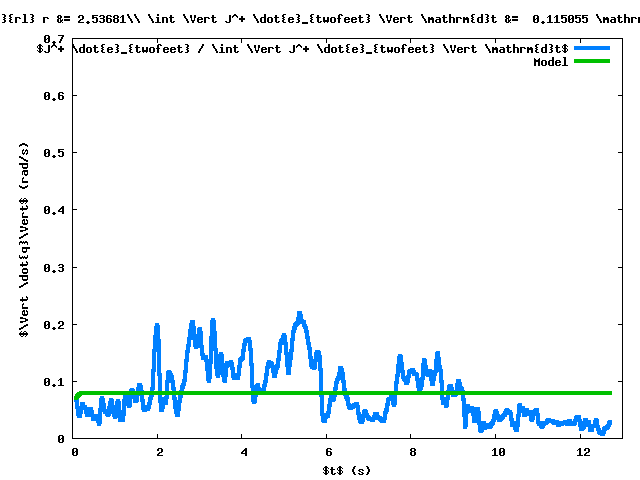
\includegraphics{img/exp1/R/invJerror_taskTwofeet_0}}%
    \gplfronttext
  \end{picture}%
\endgroup

    }                           &
  \resizebox{.4\textwidth}{!} {
	% GNUPLOT: LaTeX picture with Postscript
\begingroup
  \makeatletter
  \providecommand\color[2][]{%
    \GenericError{(gnuplot) \space\space\space\@spaces}{%
      Package color not loaded in conjunction with
      terminal option `colourtext'%
    }{See the gnuplot documentation for explanation.%
    }{Either use 'blacktext' in gnuplot or load the package
      color.sty in LaTeX.}%
    \renewcommand\color[2][]{}%
  }%
  \providecommand\includegraphics[2][]{%
    \GenericError{(gnuplot) \space\space\space\@spaces}{%
      Package graphicx or graphics not loaded%
    }{See the gnuplot documentation for explanation.%
    }{The gnuplot epslatex terminal needs graphicx.sty or graphics.sty.}%
    \renewcommand\includegraphics[2][]{}%
  }%
  \providecommand\rotatebox[2]{#2}%
  \@ifundefined{ifGPcolor}{%
    \newif\ifGPcolor
    \GPcolortrue
  }{}%
  \@ifundefined{ifGPblacktext}{%
    \newif\ifGPblacktext
    \GPblacktexttrue
  }{}%
  % define a \g@addto@macro without @ in the name:
  \let\gplgaddtomacro\g@addto@macro
  % define empty templates for all commands taking text:
  \gdef\gplbacktext{}%
  \gdef\gplfronttext{}%
  \makeatother
  \ifGPblacktext
    % no textcolor at all
    \def\colorrgb#1{}%
    \def\colorgray#1{}%
  \else
    % gray or color?
    \ifGPcolor
      \def\colorrgb#1{\color[rgb]{#1}}%
      \def\colorgray#1{\color[gray]{#1}}%
      \expandafter\def\csname LTw\endcsname{\color{white}}%
      \expandafter\def\csname LTb\endcsname{\color{black}}%
      \expandafter\def\csname LTa\endcsname{\color{black}}%
      \expandafter\def\csname LT0\endcsname{\color[rgb]{1,0,0}}%
      \expandafter\def\csname LT1\endcsname{\color[rgb]{0,1,0}}%
      \expandafter\def\csname LT2\endcsname{\color[rgb]{0,0,1}}%
      \expandafter\def\csname LT3\endcsname{\color[rgb]{1,0,1}}%
      \expandafter\def\csname LT4\endcsname{\color[rgb]{0,1,1}}%
      \expandafter\def\csname LT5\endcsname{\color[rgb]{1,1,0}}%
      \expandafter\def\csname LT6\endcsname{\color[rgb]{0,0,0}}%
      \expandafter\def\csname LT7\endcsname{\color[rgb]{1,0.3,0}}%
      \expandafter\def\csname LT8\endcsname{\color[rgb]{0.5,0.5,0.5}}%
    \else
      % gray
      \def\colorrgb#1{\color{black}}%
      \def\colorgray#1{\color[gray]{#1}}%
      \expandafter\def\csname LTw\endcsname{\color{white}}%
      \expandafter\def\csname LTb\endcsname{\color{black}}%
      \expandafter\def\csname LTa\endcsname{\color{black}}%
      \expandafter\def\csname LT0\endcsname{\color{black}}%
      \expandafter\def\csname LT1\endcsname{\color{black}}%
      \expandafter\def\csname LT2\endcsname{\color{black}}%
      \expandafter\def\csname LT3\endcsname{\color{black}}%
      \expandafter\def\csname LT4\endcsname{\color{black}}%
      \expandafter\def\csname LT5\endcsname{\color{black}}%
      \expandafter\def\csname LT6\endcsname{\color{black}}%
      \expandafter\def\csname LT7\endcsname{\color{black}}%
      \expandafter\def\csname LT8\endcsname{\color{black}}%
    \fi
  \fi
  \setlength{\unitlength}{0.0500bp}%
  \begin{picture}(7200.00,5040.00)%
    \gplgaddtomacro\gplbacktext{%
      \csname LTb\endcsname%
      \put(1342,704){\makebox(0,0)[r]{\strut{} 0}}%
      \put(1342,1194){\makebox(0,0)[r]{\strut{} 0.01}}%
      \put(1342,1684){\makebox(0,0)[r]{\strut{} 0.02}}%
      \put(1342,2174){\makebox(0,0)[r]{\strut{} 0.03}}%
      \put(1342,2665){\makebox(0,0)[r]{\strut{} 0.04}}%
      \put(1342,3155){\makebox(0,0)[r]{\strut{} 0.05}}%
      \put(1342,3645){\makebox(0,0)[r]{\strut{} 0.06}}%
      \put(1342,4135){\makebox(0,0)[r]{\strut{} 0.07}}%
      \put(1474,484){\makebox(0,0){\strut{} 0}}%
      \put(2245,484){\makebox(0,0){\strut{} 2}}%
      \put(3016,484){\makebox(0,0){\strut{} 4}}%
      \put(3787,484){\makebox(0,0){\strut{} 6}}%
      \put(4557,484){\makebox(0,0){\strut{} 8}}%
      \put(5328,484){\makebox(0,0){\strut{} 10}}%
      \put(6099,484){\makebox(0,0){\strut{} 12}}%
      \put(6870,484){\makebox(0,0){\strut{} 14}}%
      \put(440,2542){\rotatebox{90}{\makebox(0,0){\strut{}$\Vert \dot{q}\Vert$ (rad/s)}}}%
      \put(4172,154){\makebox(0,0){\strut{}$t$ (s)}}%
      \put(4172,4710){\makebox(0,0){\strut{}Right and left hand motion - Twofeet task}}%
    }%
    \gplgaddtomacro\gplfronttext{%
      \csname LTb\endcsname%
      \put(5883,4207){\makebox(0,0)[r]{\strut{}$J^+ \dot{e}_{twofeet}$}}%
      \csname LTb\endcsname%
      \put(5883,3987){\makebox(0,0)[r]{\strut{}Model}}%
    }%
    \gplbacktext
    \put(0,0){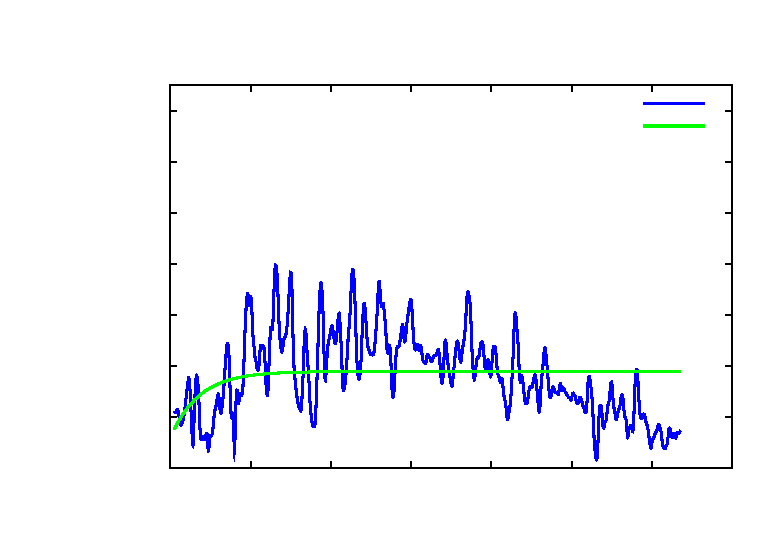
\includegraphics{img/exp1/RL/invJerror_taskTwofeet_0}}%
    \gplfronttext
  \end{picture}%
\endgroup

    }\\
  $r = 0.530217 $ & $r = 0.394636$\\
\end{tabular*}
\caption{Comparison of the fitting for the \emph{two feet} task for the \emph{both hands} and \emph{right hand} motion at the first iteration of the identification algorithm.
The residues $r$ of the optimizations are showed in the second row.}
\label{fig:exp1:taskTwofeet0}
\end{figure*}

\end{document}
